




%- HandOut Flag -----------------------------------------------------------------------------------------
\newif\ifHandout
%	\Handouttrue  %uncomment for the printable version

%- D0cum3nt ----------------------------------------------------------------------------------------------
\documentclass[beamer,handout,10pt]{standalone}   
\ifHandout
	\setbeameroption{show notes} %print notes   
\fi

	
%- Packages ----------------------------------------------------------------------------------------------
\usepackage{custom-style}
\usepackage{math}

%--Beamer Style-----------------------------------------------------------------------------------------------
\usetheme{toninus}


\renewcommand{\action}{\curvearrowright} 
\makeatletter
\def\blfootnote{\gdef\@thefnmark{}\@footnotetext}
\makeatother





%--------------------------------------------------------------------------------------------------
%- D0cum3nt ----------------------------------------------------------------------------------------------------------------------------------
\begin{document}
%------------------------------------------------------------------------------------------------

%------------------------------------------------------------------------------------------------
\begin{frame}{Symplectic geometry (mechanics flavour)}
	\begin{columns}[T]
		\begin{column}{.50\linewidth}
			\centering
			\textit{ "geometric approach" to mechanics \dots}
			%
			\begin{columns}
				\begin{column}{.60\linewidth}
					\begin{center}
						\includegraphics[width=0.6\linewidth]{Pictures/pendulum13}			
					\end{center}
				\end{column}	
				\begin{column}{.40\linewidth}
					\begin{center}
						\includegraphics[width=0.45\linewidth]{Pictures/pendulum-phase-space}			
					\end{center}
				\end{column}	
			\end{columns}
			%
			\begin{defblock}[Symplectic Manifold]
				\vspace{-1em}
				\includestandalone[width=1\textwidth]{Pictures/Figure_sym}	
			\end{defblock}
			%
			\pause
			\begin{exblock}[$M = T^\ast Q$ is symplectic]
				with $\omega = d \theta $ given by
				$$ \left.\theta\right\vert_{(q,p)} (v) = p (\pi_\ast v) ~.$$
			\end{exblock}
			%
			\pause
			\vspace{1.2em}
			\centering
			\textit{ based on the notion of \\"states".}		
		\end{column}
		\onslide<1->{\vrule{}}
		\pause
		\begin{column}{.50\linewidth}
			\centering
			\textit{ "algebraic approach" to mechanics \dots}
			\vspace{.5em}	
			\begin{defblock}[Classical Observables]
				Unital, associative, commutative algebra $C^\infty(M)$.
			\end{defblock}
			%
			\vspace{.1em}
			\pause
			\begin{defblock}[Hamiltonian vector fields]
				$\vHam_f \in \mathfrak{X}(M)$ such that:
				$$\iota_{\vHam_f} \omega = -df \quad$$ %$\in B^1(M)$
				%
				\footnotetext{	$\vHam_f$ = \emph{Ham.v.f. pertaining to $f\in C^\infty(M)$}.}
			\end{defblock}
			\vspace{.1em}
			%
			\begin{defblock}[Poisson Algebra of Observables]
				$C^\infty(M)$ is a Poisson algebra with
				$$\{f,g\} = \iota_{\vHam_g} \iota_{\vHam_f} \omega = \omega(\vHam_f,\vHam_g) ~.$$
			\end{defblock}
			%
			\pause
			\vspace{.15em}
			\centering
			\textit{ based on the notion of \\"measurable quantities".}						
		\end{column}
	\end{columns}
	\end{frame}
	\note[itemize]{
		\footnotesize
	
		\item We work in the framework of multisymplectic geometry which is one of the possible generalizations of the well-established field of symplectic geometry.
		
		\item To recall what symplectic geometry is let me assume a particular point of view: mechanics.
		\\
		Idea:"
		Symplectic geometry is a branch of differential geometry studying symplectic manifolds; it originated as a formalization of the mathematical apparatus of classical mechanics and geometric optics."{\href{https://ncatlab.org/nlab/show/symplectic+geometry}{nlab}}
		
		Namely, a sym. mfd. is the geometric structure encoding the phase space of conservative, ordinary, classical, mechanical systems.
		
		\item $\theta$ = \emph{tautological 1-form}.
			$\theta$ evaluated at $p\in T^*Q$ in the fibre of $q\in Q$ and contracted with $v$ coincides with the form $p$ evaluated at $q$ and contracted with the push forward of $v$.
		
		\item We identify a special class of vector fields.
			Out of them one can define a Lie bracket.
		
		\item Poisson is a Lie algebra with the extra property of compatibility with the associative product (Leibniz rule)
		
		\item take away message: geometric (based on "states") vs algebraic (based on "measurable quantities").7
	}
	%------------------------------------------------------------------------------------------------
	
	%------------------------------------------------------------------------------------------------
	\begin{frame}{Reminder: momentum maps in symplectic geometry}\label{frame:symplecticmomaps}
		Consider $\theta:G\curvearrowright M$ symplectic,~~ $\underline{\cdot}:\mathfrak{g}\to \mathfrak{X}(M)$ infinitesimal action.
		\vfill
	
		\begin{columns}[T]
			\setlength{\belowdisplayskip}{5pt}
			\begin{column}{.50\linewidth}
				%
				\centering \it
				\onslide<2->{
					\begin{defblock}[Equivariant moment map]
						Smooth map $$\mu:M\to \mathfrak{g}^\ast$$
						such that:
						\begin{itemize}
							\item[i.] $d\langle \mu,\xi\rangle = -\iota_{\underline{\xi}}\omega$ 
							~\qquad, $\forall \xi \in \mathfrak{g}$
							\item[ii.] $\mu \circ \theta_g = Ad_g^\ast \circ \mu$
							 \qquad\small, $\forall g \in G$
						\end{itemize}
					\end{defblock}
				}
			\end{column}	
			%
			\onslide<2->{\vrule{}}
			%
			\begin{column}{.50\linewidth}
				\onslide<3->{			
					\begin{defblock}[Comoment map]
						Linear map $$\widetilde{\mu}: \mathfrak{g}\to C^\infty(M,\omega)$$
						such that:
						\begin{itemize}
							\item[i.] $d\widetilde{\mu}(\xi) = -\iota_{\underline{\xi}}\omega$ 
							\qquad~\small, $\forall \xi \in \mathfrak{g}$
							\item[ii.] $\widetilde{\mu}([\xi,\eta]) = \lbrace\widetilde{\mu}(\xi),\widetilde{\mu}(\eta)\rbrace$ \small, $\forall \xi,\eta \in \mathfrak{g}$
						\end{itemize}
					\end{defblock}
				}
			\end{column}	
		\end{columns}	
		%
		\pause
		\vspace{1em}
		%
		\begin{columns}[]
			\setlength{\belowdisplayskip}{5pt}
			\begin{column}{.40\linewidth}
				%
				\centering \it
				\onslide<5->{
					\begin{upshotblocktitle}[Duality]
						\begin{displaymath}
							\mu(x) : \mathfrak{\xi} \mapsto \widetilde{\mu}(\xi)\big\vert_x
						\end{displaymath}
						%
						\emph{
						\small
						"duality wrt. the currying operation"					
						}
					\end{upshotblocktitle}
				}
			\end{column}	
			%
			%
			\begin{column}{.60\linewidth}
				\onslide<4->{			
					\begin{upshotblocktitle}[$\widetilde{\mu}$ as a lift]
						\begin{displaymath}
							\begin{tikzcd}[ampersand replacement = \&]
							 \& C^\infty(M,\omega) \ar[d,"\vHam"]
							 \\
							 \mathfrak{g} \ar[ur,dashed,sloped,"\widetilde{\mu}"]\ar[r,"\underline{\cdot}"'] \& \mathfrak{X}(M)
							\end{tikzcd}
						\end{displaymath}
						%
						\emph{
						\small
						"it is a lift (in the Lie category) of the infinitesimal action by the assigment of hamiltonian v.fields."					
						}
					\end{upshotblocktitle}
				}
			\end{column}	
		\end{columns}		
	\end{frame}
	\note[itemize]{
		\item consider an action preserving the symplectic form.
		\item[-] $\langle \cdot, \cdot \rangle$ is the natural pairing of $\mathfrak{g}$ and $\mathfrak{g}^\ast$.
			\item[-] $\theta_g$ is the diffeomorphism associated to $g\in G$ via $\theta:G\curvearrowright M$
			\item[-] $Ad^\ast_g$ is the coadjoint action $G\curvearrowright \mathfrak{g}^\ast$
		\item The moment map can be reexpressed as a comomentum map.
		\item Observe that ii. on the left always implies ii. on the right. The converse is trure only if $G$ is connected.
		\item $G\curvearrowright M$ is said "Hamiltonian" (see slide \ref{frame:gisthamaction} in appendix) iff $\exists$ comoment map $\widetilde{\mu}$.
		\item \emph{moment map: Describe ${\color{orange}G\curvearrowright M}$ in terms of $\color{blue}C^\infty(M)\to\X(M)$.}
		\begin{center}
		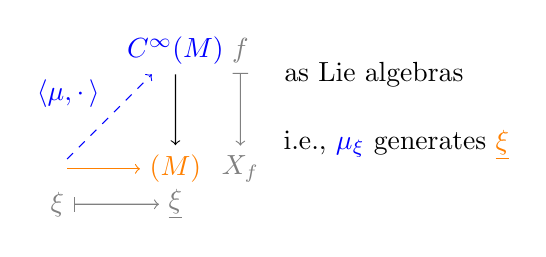
\begin{tikzpicture}[scale=1.5]
			\node[orange] (A) at (0,0) {$\g$};
			\node[gray] (A1) at (0,-.3) {$\xi$};
			\node[blue] (B) at (1,1) {$C^\infty(M)$};
			\node[gray] (B2) at (1.55,1) {$f$};
			\node[orange] (C) at (1,0) {$\X(M)$};
			\node[gray] (C1) at (1,-.3) {$\underline\xi$};
			\node[gray] (C2) at (1.55,0) {$X_f$};
	
			\path[->,blue,dashed] (A) edge node[above left] {$\langle\mu,\cdot\,\rangle$} (B);
			\path[->,orange] (A) edge (C);
			\path[->] (B) edge (C);
			\path[|->,gray] (A1) edge (C1);
			\path[|->,gray] (B2) edge (C2);
	
			\begin{scope}[xshift=3cm]
				\node at (-.32,.8) {as Lie algebras};
				\node at (-.13,.2) {i.e., {\color{blue}$\mu_\xi$} generates {\color{orange}$\underline\xi$}};
			\end{scope}
		\end{tikzpicture}
		
			\footnotesize		(\emph{moment map:} ${\color{blue}\mu:M\to\g^*}$, 
		 \emph{Hamiltonian $G$-space:} 	$(M,\omega,G,\mu)$)
		\end{center}
		\item
		 $\alpha\mapsto X_\alpha$ is a homomorphism of Leibniz algebras:
		$$\d\{\alpha,\beta\} = \d\L_{X_\alpha}\beta = \L_{X_\alpha}\iota_{X_\beta}\omega = \iota_{[X_\alpha,X_\beta]}\omega ~{\color{black!80} \implies}~
		X_{\{\alpha,\beta\}} = [X_\alpha,X_\beta]$$
	}
	%------------------------------------------------------------------------------------------------
	
	\subsection{Regular reduction}
	%------------------------------------------------------------------------------------------------
	\begin{frame}{Regular reduction in symplectic geometry}
		\textbf{\color{UniGreen}Symplectic reduction:}~~
		\\ 
		{\it \small
		Procedure associating to any (suitably regular) pair of symplectic manifold and Hamiltonian action another symplectic manifold of smaller dimension.}
		\vfill
		\pause
		\begin{thmblock}[Marsden-Weinstein reduction \cite{MarsdenWeinstein74}]
			\vspace{-.4em}\hspace{-1em}
			\begin{tabular}{l p{14cm}}
				Given: & $(M,\omega)$ symplectic
				\\
				& $G\curvearrowright M$ symplectic with equivariant momap. $\mu:M\to \mathfrak{g}^*$
				\\[.2em]
				Assume: & $\phi \in \mathfrak{g}^*$ regular value of $\mu$ 
				\qquad\quad \footnotesize \textcolor{gray}{($\Rightarrow$ $\mu^{-1}(\phi)\hookrightarrow M$ smooth embedding)}
				\\
				& $G_\phi\curvearrowright \mu^{-1}(\phi)$ free and proper
				\quad \footnotesize \textcolor{gray}{($\Rightarrow$ $\mu^{-1}(\phi)/G_\phi$ smooth manifold)}
				\\[.4em]
				Then: & $\exists!$ symplectic structure $\omega_\phi$ in $M_\phi:= \mu^{-1}(\phi)/G_\phi$ \\
				& s.t. $\pi^\ast \omega_\phi = j^\ast \omega$ 
				\qquad {\footnotesize with $j:\mu^{-1}(\phi) \hookrightarrow M$ and $\pi:\mu^{-1}(\phi)\twoheadrightarrow M_\mu$}
			\end{tabular}
			\vspace{-.4em}
		\end{thmblock}
		%
		\vfill
		\pause
		\begin{columns}
			\begin{column}{0.40\textwidth}
				\includegraphics[width=\textwidth]{Pictures/Reduction}
			\end{column}	
			
			\begin{column}{0.6\textwidth}
					\textbf{\color{UniGreen}In mechanics:}~~
					\\
				{\it \small
					it embodies the process of restricting the dynamics of the system to the level sets of the conserved quantities pertaining to the symmetry group.		
				}
				\\[.2em]
				\color{gray}\small( e.g. restricting to studying a point-like particle in a central potential by studying it in radial coordinates)
			\end{column}	
		\end{columns}	
	\end{frame}
	\note[itemize]{
		\item {Symplectic Reduction} takes two inputs:
		\\ 1. Hamiltonian $G$-space $(M,\omega,{\color{orange}G},{\color{blue}\mu})$
		\\ 2. parameter ${\color{blue}\phi}\in\g^*$
		\item The \emph{reduced space} is $M_\phi:={\color{blue}\mu^{-1}(\phi)}{\color{orange}/G_\phi}$.
		\item (Marsden--Weinstein '74, Meyer '73) THM:\\
			If $\mu^{-1}(\phi)\subset M$ is smooth and $G_\phi\curvearrowright \mu^{-1}(\phi)$ is free and proper, then there is a \textbf{unique symplectic form} $\omega_\phi\in\Omega^2(M_\phi)$ such that $\pi^*\omega_\phi = i^*\omega$.
	
	
		\begin{center}
		\begin{tikzpicture}[scale=2]
			\node[blue] (A) at (0,0) {$\mu^{-1}(\phi)$};
			\node[gray] (A1) at (0,.3) {$i^*\omega$};
			\node[gray] (A2) at (-.6,0) {$\pi^*\omega_\phi$};
			\node[blue] (B) at (1,0) {$M$};
			\node[gray] (B1) at (1,.3) {$\omega$};
			\node[orange] (C) at (0,-.8) {$M_\phi$};
			\node[gray] (C2) at (-.6,-.8) {$\omega_\phi$};
	
			\path[right hook->,blue] (A) edge node[above] {$i$} (B);
			\path[orange,->] (A) edge node[left] {$\pi$} (C);
			\begin{scope}[xshift=-1.8cm]
				\node[blue] at (0,0) {\small restrict to $\{\mu=\phi\}$};
				\node[orange] at (.15,-.4) {\small quotient by $G_\phi$};
			\end{scope}
		\end{tikzpicture}
		\end{center}
		\item Heuristic Approach to Reduction:
		\\1. describe $G\curvearrowright M$ in terms of $\omega$ 	\hspace{1cm}
		({\color{green}moment map $\mu$})
		\\2. identify a distinguished reduced space \hspace{1cm}
		({\color{green}reduction at $\mu=0$})
		\\3. use the ambiguity in 1.\ to obtain a family of reduced spaces \hspace{1cm}
		({\color{green}reduction at $\mu-\phi=0$, i.e.\ reduction at $\mu=\phi$}
		\\
		{\tiny Note: If $G_\phi\neq G$, then $\mu-\phi:M\to\g^*$ is not a moment map for either $G\curvearrowright M$ or $G_\phi\curvearrowright M$.}
		
	}
	%------------------------------------------------------------------------------------------------
	
	%------------------------------------------------------------------------------------------------
	\subsection{Singular reduction}
	\begin{frame}{Symplectic singular reduction schemes}
		\begin{block}{The gist of singular reduction}
			 \begin{itemize}
				 \item[-] when $\mu$ is singular (i.e. $\mu^{-1}(0)$ is not a mfd.), the (geometrically) reduced space may not exist.
				 \item[-] a \emph{singular reduction scheme} is a procedure to construct a "reduced" algebra of observable out of the given data
				 \item[-] such that it corresponds to the algebra of observable of the reduced manifold in the regular case.
			 \end{itemize}
		\end{block}
		 %
		 \pause
		 %
		\begin{thmblock}[Sniatycki-Weinstein reduction \cite{SniatyckiWeinstein83}]
			\vspace{-.4em}\hspace{-1em}
			\begin{tabular}{l p{14cm}}
				Given: & $(M,\omega)$ symplectic
				\\
				& $G\curvearrowright M$ symplectic with equivariant momap. $\mu:M\to \mathfrak{g}^*$
				\\[.4em]
				Then: & 
				$\displaystyle \left[\sfrac{C^\infty(M)}{I_\mu}\right]^G$
				admits a Poisson algebra structure 
				\blfootnote{$I_\mu$ = associative ideal generated by $\widetilde{\mu}(\g)$}			
				\\
				& it agrees with the M--W reduction in the regular case.		
			\end{tabular}
			\vspace{-.4em}
		\end{thmblock}
	 
	
	\end{frame}
	\note[itemize]{
	 \item Let $(M,\omega,G,\mu)$ be a symplectic Hamiltonian $G$-space.
	 \item The \emph{momentum ideal} is the associative ideal $I_\mu\subset C^\infty(M)$ generated by the momenta $\mu_{\xi}$ for any $\xi\in \mathfrak{g}$.
			Namely
			\[
				I_\mu 
				= 
				\Big\langle \mu_\xi \Big\rangle_{\xi \in \mathfrak{g}}^{\text{\tiny asso.}} 
				=
				\left\{
					\left.
						\sum_{i=1}^n f_i ~ \mu_{\xi_i}
					\right|~
						f_i \in C^\infty(M),~ \xi_i\in \mathfrak{g},~  1 \leq i \leq n
				\right\}
			\]
	
	 \item The \emph{\'Sniatycki--Weinstein reduction} is the Poisson algebra
			\[
				\left(C^\infty(M)/I_\mu\right)^G.
			\]
	
	
	}
	%------------------------------------------------------------------------------------------------
	

	%------------------------------------------------------------------------------------------------
\ifstandalone
\begin{frame}[t,allowframebreaks]{Extended Bibliography}
	\nocite{*}
	\bibliographystyle{alpha}
	\bibliography{bibfile}
\end{frame}
\fi
%------------------------------------------------------------------------------------------------


%------------------------------------------------------------------------------------------------
\end{document}